\documentclass{beamer}
\usetheme{Warsaw}
\usepackage{polski}
\usepackage[utf8]{inputenc}
\usepackage{verbatim}
\usepackage{graphicx}
\title
{Octopus}
\subtitle{multiplayer, casual, 2D shooter}
\author[]
{Bujok Mikołaj \and Kubiak Jakub \\ \and Szymon Miękus\and Nikodem Adrian}
\date[\today]
{Projekt zespołowy 2013}
\subject{Informatyka}

\begin{document}
%first frame
\frame{\titlepage}
\begin{frame}
  \frametitle{Agenda}
  \begin{itemize}
  \item O grze
  \item Architektura
  \item Implementacja
  \item Plany
  \item Informacje
  \end{itemize}
\end{frame}

% frame
\begin{frame}
  \frametitle{O grze}
  \begin{itemize}
    \item Reguły są proste - dwu wymiarowy DeathMatch
    \item Drużyny zaczynają na przeciwległych końcach mapy
    \item Mapy są symetryczne - zapewnia to zbalansowanie
          szans na poziomie architektury gry
    \item Na mapie losowo pojawiają się bonusy (chwilowe przyspieszanie, lepsza broń itp.
    \item Wygrywa ta drużna, która 'pozbędzie się' wszystkich przeciwników
  \end{itemize}
\end{frame}

% frame
\begin{frame}
\begin{figure}[ht]

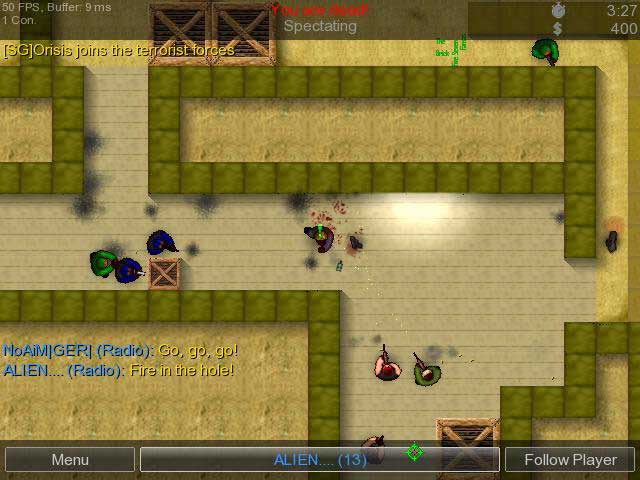
\includegraphics[scale=0.4]{cs2d.jpg}
\label{cs2d}
\caption{\href{http://www.unrealsoftware.de}{http://www.unrealsoftware.de}}
\end{figure}
\end{frame}
\end{document}
